\section{Qt\-File\-Icon\-View\-Item Class Reference}
\label{classQtFileIconViewItem}\index{QtFileIconViewItem@{QtFileIconViewItem}}
{\tt \#include $<$qfileiconview.h$>$}

\subsection*{Public Types}
\begin{CompactItemize}
\item 
enum {\bf Item\-Type} \{ {\bf File} =  0, 
{\bf Dir}, 
{\bf Link}, 
{\bf Image}
 \}
\end{CompactItemize}
\subsection*{Public Member Functions}
\begin{CompactItemize}
\item 
{\bf Qt\-File\-Icon\-View\-Item} ({\bf Qt\-File\-Icon\-View} $\ast$parent, QFile\-Info $\ast$fi, int pixindex)
\item 
virtual {\bf $\sim$Qt\-File\-Icon\-View\-Item} ()
\item 
{\bf Item\-Type} {\bf type} () const 
\item 
QString {\bf filename} () const 
\item 
virtual bool {\bf accept\-Drop} (const QMime\-Source $\ast$e) const 
\item 
virtual void {\bf set\-Text} (const QString \&text)
\item 
virtual QPixmap $\ast$ {\bf pixmap} () const 
\item 
virtual void {\bf drag\-Entered} ()
\item 
virtual void {\bf drag\-Left} ()
\item 
void {\bf view\-Mode\-Changed} ({\bf Qt\-File\-Icon\-View::View\-Mode} m)
\item 
void {\bf paint\-Item} (QPainter $\ast$p, const QColor\-Group \&cg)
\end{CompactItemize}
\subsection*{Public Attributes}
\begin{CompactItemize}
\item 
QPixmap {\bf img}
\item 
QPixmap $\ast$ {\bf p\_\-img}
\end{CompactItemize}
\subsection*{Protected Member Functions}
\begin{CompactItemize}
\item 
virtual void {\bf dropped} (QDrop\-Event $\ast$e, const QValue\-List$<$ QIcon\-Drag\-Item $>$ \&)
\end{CompactItemize}
\subsection*{Protected Attributes}
\begin{CompactItemize}
\item 
QString {\bf item\-File\-Name}
\item 
QFile\-Info $\ast$ {\bf item\-File\-Info}
\item 
{\bf Item\-Type} {\bf item\-Type}
\item 
bool {\bf check\-Set\-Text}
\item 
QTimer {\bf timer}
\item 
{\bf Qt\-File\-Icon\-View::View\-Mode} {\bf vm}
\item 
int {\bf Pix\-Index}
\end{CompactItemize}
\subsection*{Friends}
\begin{CompactItemize}
\item 
class {\bf Qt\-File\-Icon\-View}
\end{CompactItemize}


\subsection{Member Enumeration Documentation}
\index{QtFileIconViewItem@{Qt\-File\-Icon\-View\-Item}!ItemType@{ItemType}}
\index{ItemType@{ItemType}!QtFileIconViewItem@{Qt\-File\-Icon\-View\-Item}}
\subsubsection{\setlength{\rightskip}{0pt plus 5cm}enum {\bf Qt\-File\-Icon\-View\-Item::Item\-Type}}\label{classQtFileIconViewItem_QtFileIconViewItemw4}


\begin{Desc}
\item[Enumeration values: ]\par
\begin{description}
\index{File@{File}!QtFileIconViewItem@{QtFileIconViewItem}}\index{QtFileIconViewItem@{QtFileIconViewItem}!File@{File}}\item[{\em 
File\label{classQtFileIconViewItem_QtFileIconViewItemw4QtFileIconViewItemw0}
}]\index{Dir@{Dir}!QtFileIconViewItem@{QtFileIconViewItem}}\index{QtFileIconViewItem@{QtFileIconViewItem}!Dir@{Dir}}\item[{\em 
Dir\label{classQtFileIconViewItem_QtFileIconViewItemw4QtFileIconViewItemw1}
}]\index{Link@{Link}!QtFileIconViewItem@{QtFileIconViewItem}}\index{QtFileIconViewItem@{QtFileIconViewItem}!Link@{Link}}\item[{\em 
Link\label{classQtFileIconViewItem_QtFileIconViewItemw4QtFileIconViewItemw2}
}]\index{Image@{Image}!QtFileIconViewItem@{QtFileIconViewItem}}\index{QtFileIconViewItem@{QtFileIconViewItem}!Image@{Image}}\item[{\em 
Image\label{classQtFileIconViewItem_QtFileIconViewItemw4QtFileIconViewItemw3}
}]\end{description}
\end{Desc}



Definition at line 141 of file qfileiconview.h.

Referenced by type().



\footnotesize\begin{verbatim}141                   {
142         File = 0,// define MP3 file
143         Dir,
144         Link,
145         Image
146     };
\end{verbatim}\normalsize 


\subsection{Constructor \& Destructor Documentation}
\index{QtFileIconViewItem@{Qt\-File\-Icon\-View\-Item}!QtFileIconViewItem@{QtFileIconViewItem}}
\index{QtFileIconViewItem@{QtFileIconViewItem}!QtFileIconViewItem@{Qt\-File\-Icon\-View\-Item}}
\subsubsection{\setlength{\rightskip}{0pt plus 5cm}Qt\-File\-Icon\-View\-Item::Qt\-File\-Icon\-View\-Item ({\bf Qt\-File\-Icon\-View} $\ast$ {\em parent}, QFile\-Info $\ast$ {\em fi}, int {\em pixindex})}\label{classQtFileIconViewItem_QtFileIconViewItema0}




Definition at line 98 of file qfileiconview.cpp.

References add\-Border(), Array\-Image, check\-Set\-Text, File, Image, img, item\-File\-Info, item\-File\-Name, item\-Type, and Pix\-Index.



\footnotesize\begin{verbatim}99     : QIconViewItem( parent, fi->fileName() ), itemFileName( fi->filePath() ),PixIndex(pixindex),
100       itemFileInfo( fi ), checkSetText( FALSE )
101 {
102     vm = QtFileIconView::Large;//view mode
103 
104    if ( itemFileInfo->isFile() )
105     {
106         if(fi->extension()=="jpg"||fi->extension()=="png"||fi->extension()=="bmp"||fi->extension()=="jpeg")
107         itemType=Image;
108         else if(fi->extension()=="mp3")
109         {
110         itemType = File;//MP3 File
111         }
112     }
113 
114     checkSetText = TRUE;
115 
116     QObject::connect( &timer, SIGNAL( timeout() ), iconView(), SLOT( openFolder() ) );
117         if(itemType==Image)
118         {
119                  if(ArrayImage[PixIndex])
120                  {
121                         delete ArrayImage[PixIndex];
122                  }
123                  img=QPixmap(itemFileName);
124                 ArrayImage[PixIndex]=addBorder(&img,1);
125                 setPixmap(*ArrayImage[PixIndex]);
126         }
127 }
\end{verbatim}\normalsize 


Here is the call graph for this function:\begin{figure}[H]
\begin{center}
\leavevmode

\includegraphics[width=166pt]{classQtFileIconViewItem_QtFileIconViewItema0_cgraph}
\end{center}
\end{figure}
\index{QtFileIconViewItem@{Qt\-File\-Icon\-View\-Item}!~QtFileIconViewItem@{$\sim$QtFileIconViewItem}}
\index{~QtFileIconViewItem@{$\sim$QtFileIconViewItem}!QtFileIconViewItem@{Qt\-File\-Icon\-View\-Item}}
\subsubsection{\setlength{\rightskip}{0pt plus 5cm}Qt\-File\-Icon\-View\-Item::$\sim${\bf Qt\-File\-Icon\-View\-Item} ()\hspace{0.3cm}{\tt  [virtual]}}\label{classQtFileIconViewItem_QtFileIconViewItema1}




Definition at line 161 of file qfileiconview.cpp.

References item\-File\-Info.



\footnotesize\begin{verbatim}162 {
163     delete itemFileInfo;
164 }
\end{verbatim}\normalsize 


\subsection{Member Function Documentation}
\index{QtFileIconViewItem@{Qt\-File\-Icon\-View\-Item}!acceptDrop@{acceptDrop}}
\index{acceptDrop@{acceptDrop}!QtFileIconViewItem@{Qt\-File\-Icon\-View\-Item}}
\subsubsection{\setlength{\rightskip}{0pt plus 5cm}bool Qt\-File\-Icon\-View\-Item::accept\-Drop (const QMime\-Source $\ast$ {\em e}) const\hspace{0.3cm}{\tt  [virtual]}}\label{classQtFileIconViewItem_QtFileIconViewItema4}




Definition at line 209 of file qfileiconview.cpp.

References Dir, and type().



\footnotesize\begin{verbatim}210 {
211     if ( type() == Dir && e->provides( "text/uri-list" ) &&
212          dropEnabled() )
213         return TRUE;
214 
215     return FALSE;
216 }
\end{verbatim}\normalsize 


Here is the call graph for this function:\begin{figure}[H]
\begin{center}
\leavevmode

\includegraphics[width=180pt]{classQtFileIconViewItem_QtFileIconViewItema4_cgraph}
\end{center}
\end{figure}
\index{QtFileIconViewItem@{Qt\-File\-Icon\-View\-Item}!dragEntered@{dragEntered}}
\index{dragEntered@{dragEntered}!QtFileIconViewItem@{Qt\-File\-Icon\-View\-Item}}
\subsubsection{\setlength{\rightskip}{0pt plus 5cm}void Qt\-File\-Icon\-View\-Item::drag\-Entered ()\hspace{0.3cm}{\tt  [virtual]}}\label{classQtFileIconViewItem_QtFileIconViewItema7}




Definition at line 247 of file qfileiconview.cpp.

References Dir, item\-File\-Name, and type().



\footnotesize\begin{verbatim}248 {
249     if ( type() != Dir ||
250          type() == Dir && !QDir( itemFileName ).isReadable() )
251         return;
252 
253     ( (QtFileIconView*)iconView() )->setOpenItem( this );
254     timer.start( 1500 );
255 }
\end{verbatim}\normalsize 


Here is the call graph for this function:\begin{figure}[H]
\begin{center}
\leavevmode

\includegraphics[width=182pt]{classQtFileIconViewItem_QtFileIconViewItema7_cgraph}
\end{center}
\end{figure}
\index{QtFileIconViewItem@{Qt\-File\-Icon\-View\-Item}!dragLeft@{dragLeft}}
\index{dragLeft@{dragLeft}!QtFileIconViewItem@{Qt\-File\-Icon\-View\-Item}}
\subsubsection{\setlength{\rightskip}{0pt plus 5cm}void Qt\-File\-Icon\-View\-Item::drag\-Left ()\hspace{0.3cm}{\tt  [virtual]}}\label{classQtFileIconViewItem_QtFileIconViewItema8}




Definition at line 257 of file qfileiconview.cpp.

References Dir, item\-File\-Name, and type().



\footnotesize\begin{verbatim}258 {
259     if ( type() != Dir ||
260          type() == Dir && !QDir( itemFileName ).isReadable() )
261         return;
262 
263     timer.stop();
264 }
\end{verbatim}\normalsize 


Here is the call graph for this function:\begin{figure}[H]
\begin{center}
\leavevmode
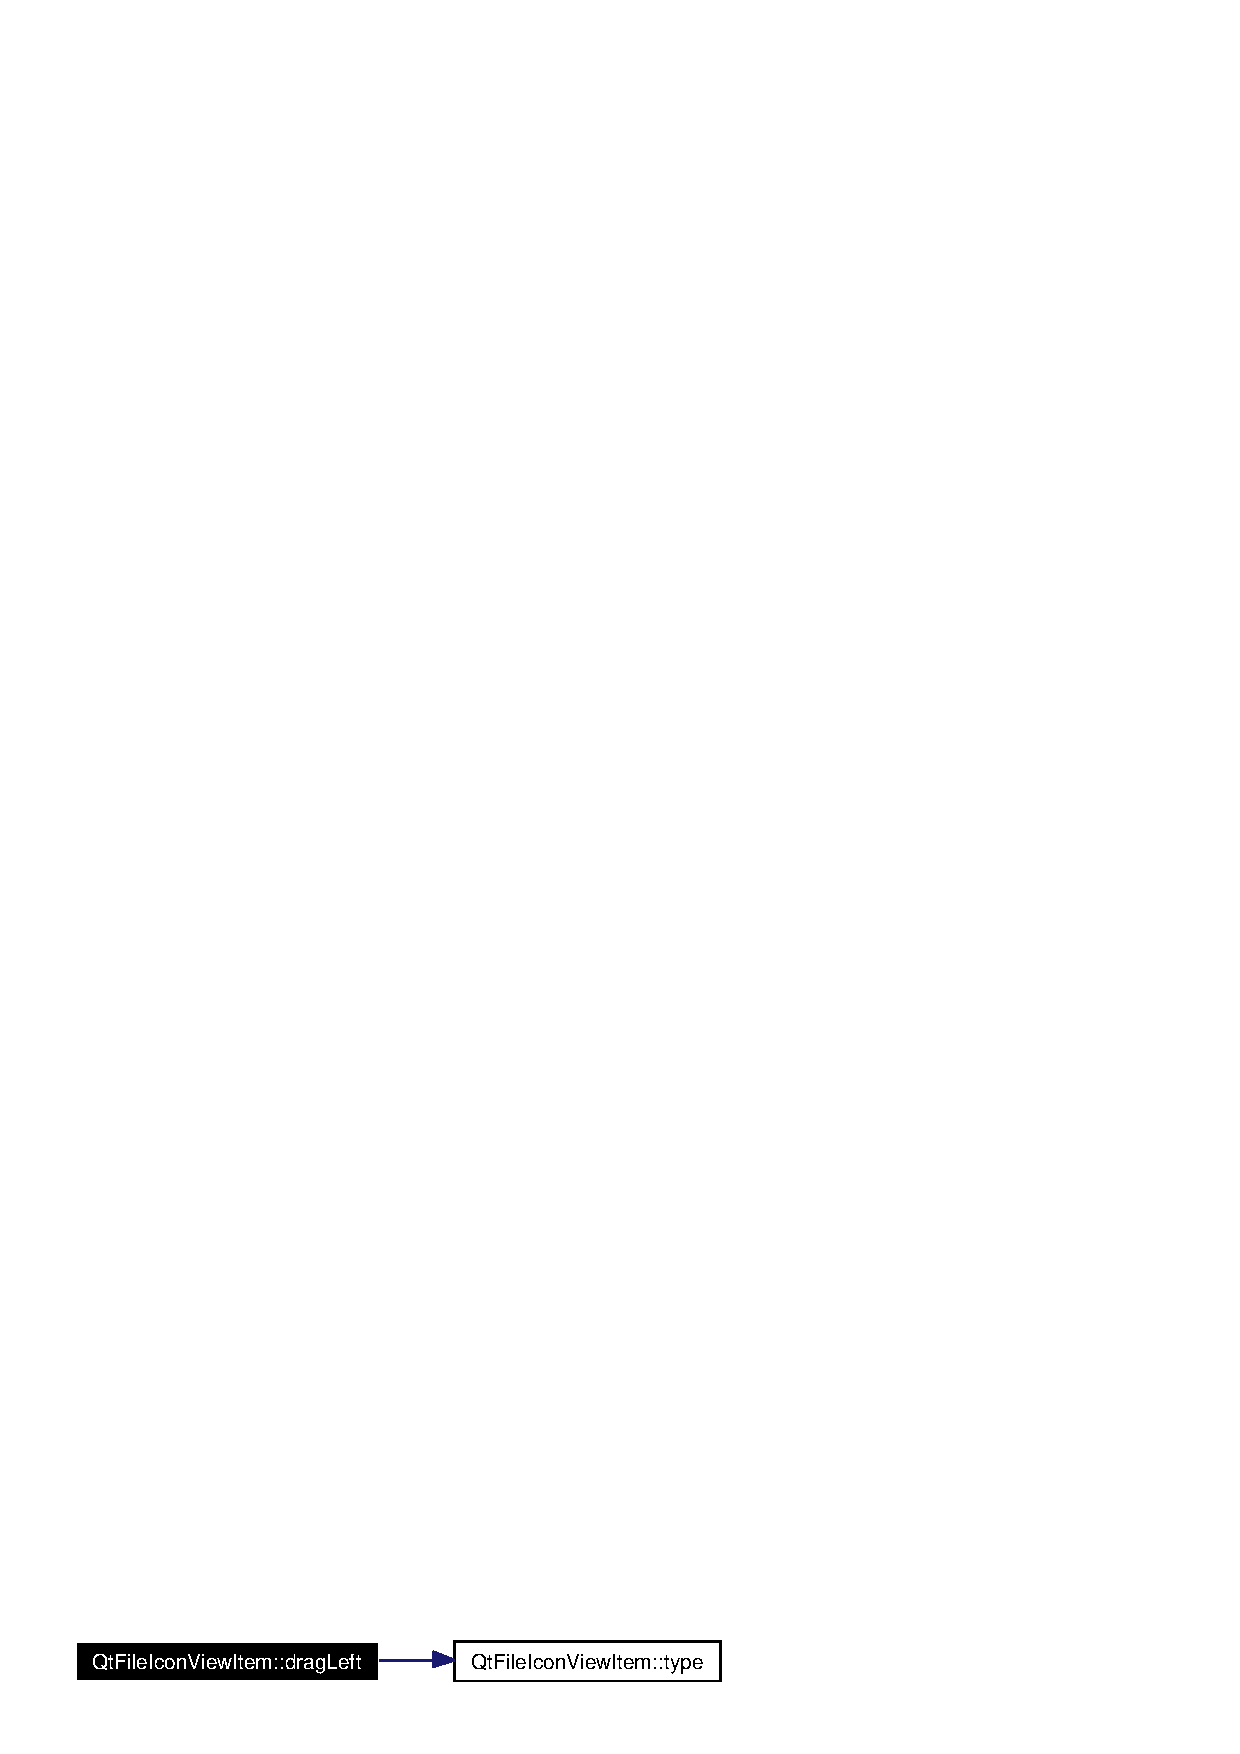
\includegraphics[width=173pt]{classQtFileIconViewItem_QtFileIconViewItema8_cgraph}
\end{center}
\end{figure}
\index{QtFileIconViewItem@{Qt\-File\-Icon\-View\-Item}!dropped@{dropped}}
\index{dropped@{dropped}!QtFileIconViewItem@{Qt\-File\-Icon\-View\-Item}}
\subsubsection{\setlength{\rightskip}{0pt plus 5cm}void Qt\-File\-Icon\-View\-Item::dropped (QDrop\-Event $\ast$ {\em e}, const QValue\-List$<$ QIcon\-Drag\-Item $>$ \&)\hspace{0.3cm}{\tt  [protected, virtual]}}\label{classQtFileIconViewItem_QtFileIconViewItemb0}




Definition at line 218 of file qfileiconview.cpp.

References filename().



\footnotesize\begin{verbatim}219 {
220     timer.stop();
221 
222     if ( !QUriDrag::canDecode( e ) ) {
223         e->ignore();
224         return;
225     }
226 
227     QStringList lst;
228     QUriDrag::decodeLocalFiles( e, lst );
229 
230     QString str;
231     if ( e->action() == QDropEvent::Copy )
232         str = "Copy\n\n";
233     else
234         str = "Move\n\n";
235     for ( uint i = 0; i < lst.count(); ++i )
236         str += QString( "   %1\n" ).arg( lst[i] );
237     str += QString( "\n"
238         "To\n\n"
239         "       %1" ).arg( filename() );
240 
241     QMessageBox::information( iconView(), e->action() == QDropEvent::Copy ? "Copy" : "Move" , str, "Not Implemented" );
242     if ( e->action() == QDropEvent::Move )
243         QMessageBox::information( iconView(), "Remove" , str, "Not Implemented" );
244     e->acceptAction();
245 }
\end{verbatim}\normalsize 


Here is the call graph for this function:\begin{figure}[H]
\begin{center}
\leavevmode

\includegraphics[width=183pt]{classQtFileIconViewItem_QtFileIconViewItemb0_cgraph}
\end{center}
\end{figure}
\index{QtFileIconViewItem@{Qt\-File\-Icon\-View\-Item}!filename@{filename}}
\index{filename@{filename}!QtFileIconViewItem@{Qt\-File\-Icon\-View\-Item}}
\subsubsection{\setlength{\rightskip}{0pt plus 5cm}QString Qt\-File\-Icon\-View\-Item::filename () const\hspace{0.3cm}{\tt  [inline]}}\label{classQtFileIconViewItem_QtFileIconViewItema3}




Definition at line 154 of file qfileiconview.h.

References item\-File\-Name.

Referenced by Qt\-File\-Icon\-View::drag\-Object(), dropped(), Qt\-File\-Icon\-View::item\-Double\-Clicked(), and Qt\-File\-Icon\-View::slot\-Delet\-Curr\-Item().



\footnotesize\begin{verbatim}154 { return itemFileName; }
\end{verbatim}\normalsize 
\index{QtFileIconViewItem@{Qt\-File\-Icon\-View\-Item}!paintItem@{paintItem}}
\index{paintItem@{paintItem}!QtFileIconViewItem@{Qt\-File\-Icon\-View\-Item}}
\subsubsection{\setlength{\rightskip}{0pt plus 5cm}void Qt\-File\-Icon\-View\-Item::paint\-Item (QPainter $\ast$ {\em p}, const QColor\-Group \& {\em cg})}\label{classQtFileIconViewItem_QtFileIconViewItema10}




Definition at line 128 of file qfileiconview.cpp.

References item\-File\-Info.



\footnotesize\begin{verbatim}129 {
130     if ( itemFileInfo->isSymLink() ) {
131         QFont f( p->font() );
132         f.setItalic( TRUE );
133         p->setFont( f );
134     }
135     QIconViewItem::paintItem( p, cg );
136 }
\end{verbatim}\normalsize 
\index{QtFileIconViewItem@{Qt\-File\-Icon\-View\-Item}!pixmap@{pixmap}}
\index{pixmap@{pixmap}!QtFileIconViewItem@{Qt\-File\-Icon\-View\-Item}}
\subsubsection{\setlength{\rightskip}{0pt plus 5cm}QPixmap $\ast$ Qt\-File\-Icon\-View\-Item::pixmap () const\hspace{0.3cm}{\tt  [virtual]}}\label{classQtFileIconViewItem_QtFileIconViewItema6}




Definition at line 145 of file qfileiconview.cpp.

References Array\-Image, icon\-File\-Large, Image, item\-Type, and Pix\-Index.



\footnotesize\begin{verbatim}146 {
147     switch ( itemType ) 
148     {
149    
150         case Image:
151         {
152                 return ArrayImage[PixIndex];
153         }
154         default:
155         {
156                 return iconFileLarge;
157         }
158     }
159 }
\end{verbatim}\normalsize 
\index{QtFileIconViewItem@{Qt\-File\-Icon\-View\-Item}!setText@{setText}}
\index{setText@{setText}!QtFileIconViewItem@{Qt\-File\-Icon\-View\-Item}}
\subsubsection{\setlength{\rightskip}{0pt plus 5cm}void Qt\-File\-Icon\-View\-Item::set\-Text (const QString \& {\em text})\hspace{0.3cm}{\tt  [virtual]}}\label{classQtFileIconViewItem_QtFileIconViewItema5}




Definition at line 166 of file qfileiconview.cpp.

References check\-Set\-Text, item\-File\-Info, and item\-File\-Name.



\footnotesize\begin{verbatim}167 {
168     if ( checkSetText ) {
169         if ( text == "." || text == "." || text.isEmpty() )
170             return;
171         QDir dir( itemFileInfo->dir() );
172         if ( dir.rename( itemFileInfo->fileName(), text ) ) {
173             itemFileName = itemFileInfo->dirPath( TRUE ) + "/" + text;
174             delete itemFileInfo;
175             itemFileInfo = new QFileInfo( itemFileName );
176             QIconViewItem::setText( text );
177         }
178     } else {
179         QIconViewItem::setText( text );
180     }
181 }
\end{verbatim}\normalsize 
\index{QtFileIconViewItem@{Qt\-File\-Icon\-View\-Item}!type@{type}}
\index{type@{type}!QtFileIconViewItem@{Qt\-File\-Icon\-View\-Item}}
\subsubsection{\setlength{\rightskip}{0pt plus 5cm}{\bf Item\-Type} Qt\-File\-Icon\-View\-Item::type () const\hspace{0.3cm}{\tt  [inline]}}\label{classQtFileIconViewItem_QtFileIconViewItema2}




Definition at line 152 of file qfileiconview.h.

References item\-Type, and Item\-Type.

Referenced by accept\-Drop(), drag\-Entered(), drag\-Left(), Qt\-File\-Icon\-View::item\-Double\-Clicked(), and Qt\-File\-Icon\-View::open\-Folder().



\footnotesize\begin{verbatim}153     { return itemType; }
\end{verbatim}\normalsize 
\index{QtFileIconViewItem@{Qt\-File\-Icon\-View\-Item}!viewModeChanged@{viewModeChanged}}
\index{viewModeChanged@{viewModeChanged}!QtFileIconViewItem@{Qt\-File\-Icon\-View\-Item}}
\subsubsection{\setlength{\rightskip}{0pt plus 5cm}void Qt\-File\-Icon\-View\-Item::view\-Mode\-Changed ({\bf Qt\-File\-Icon\-View::View\-Mode} {\em m})}\label{classQtFileIconViewItem_QtFileIconViewItema9}




Definition at line 138 of file qfileiconview.cpp.

References Dir, item\-File\-Name, and item\-Type.

Referenced by Qt\-File\-Icon\-View::set\-View\-Mode().



\footnotesize\begin{verbatim}139 {
140     vm = m;
141     setDropEnabled( itemType == Dir && QDir( itemFileName ).isReadable() );
142     calcRect();
143 }
\end{verbatim}\normalsize 


\subsection{Friends And Related Function Documentation}
\index{QtFileIconViewItem@{Qt\-File\-Icon\-View\-Item}!QtFileIconView@{QtFileIconView}}
\index{QtFileIconView@{QtFileIconView}!QtFileIconViewItem@{Qt\-File\-Icon\-View\-Item}}
\subsubsection{\setlength{\rightskip}{0pt plus 5cm}friend class {\bf Qt\-File\-Icon\-View}\hspace{0.3cm}{\tt  [friend]}}\label{classQtFileIconViewItem_QtFileIconViewItemn0}




Definition at line 138 of file qfileiconview.h.

\subsection{Member Data Documentation}
\index{QtFileIconViewItem@{Qt\-File\-Icon\-View\-Item}!checkSetText@{checkSetText}}
\index{checkSetText@{checkSetText}!QtFileIconViewItem@{Qt\-File\-Icon\-View\-Item}}
\subsubsection{\setlength{\rightskip}{0pt plus 5cm}bool {\bf Qt\-File\-Icon\-View\-Item::check\-Set\-Text}\hspace{0.3cm}{\tt  [protected]}}\label{classQtFileIconViewItem_QtFileIconViewItemp3}




Definition at line 175 of file qfileiconview.h.

Referenced by Qt\-File\-Icon\-View\-Item(), and set\-Text().\index{QtFileIconViewItem@{Qt\-File\-Icon\-View\-Item}!img@{img}}
\index{img@{img}!QtFileIconViewItem@{Qt\-File\-Icon\-View\-Item}}
\subsubsection{\setlength{\rightskip}{0pt plus 5cm}QPixmap {\bf Qt\-File\-Icon\-View\-Item::img}}\label{classQtFileIconViewItem_QtFileIconViewItemo0}




Definition at line 167 of file qfileiconview.h.

Referenced by Qt\-File\-Icon\-View\-Item().\index{QtFileIconViewItem@{Qt\-File\-Icon\-View\-Item}!itemFileInfo@{itemFileInfo}}
\index{itemFileInfo@{itemFileInfo}!QtFileIconViewItem@{Qt\-File\-Icon\-View\-Item}}
\subsubsection{\setlength{\rightskip}{0pt plus 5cm}QFile\-Info$\ast$ {\bf Qt\-File\-Icon\-View\-Item::item\-File\-Info}\hspace{0.3cm}{\tt  [protected]}}\label{classQtFileIconViewItem_QtFileIconViewItemp1}




Definition at line 173 of file qfileiconview.h.

Referenced by paint\-Item(), Qt\-File\-Icon\-View\-Item(), set\-Text(), and $\sim$Qt\-File\-Icon\-View\-Item().\index{QtFileIconViewItem@{Qt\-File\-Icon\-View\-Item}!itemFileName@{itemFileName}}
\index{itemFileName@{itemFileName}!QtFileIconViewItem@{Qt\-File\-Icon\-View\-Item}}
\subsubsection{\setlength{\rightskip}{0pt plus 5cm}QString {\bf Qt\-File\-Icon\-View\-Item::item\-File\-Name}\hspace{0.3cm}{\tt  [protected]}}\label{classQtFileIconViewItem_QtFileIconViewItemp0}




Definition at line 172 of file qfileiconview.h.

Referenced by drag\-Entered(), drag\-Left(), filename(), Qt\-File\-Icon\-View::open\-Folder(), Qt\-File\-Icon\-View\-Item(), set\-Text(), and view\-Mode\-Changed().\index{QtFileIconViewItem@{Qt\-File\-Icon\-View\-Item}!itemType@{itemType}}
\index{itemType@{itemType}!QtFileIconViewItem@{Qt\-File\-Icon\-View\-Item}}
\subsubsection{\setlength{\rightskip}{0pt plus 5cm}{\bf Item\-Type} {\bf Qt\-File\-Icon\-View\-Item::item\-Type}\hspace{0.3cm}{\tt  [protected]}}\label{classQtFileIconViewItem_QtFileIconViewItemp2}




Definition at line 174 of file qfileiconview.h.

Referenced by pixmap(), Qt\-File\-Icon\-View\-Item(), type(), and view\-Mode\-Changed().\index{QtFileIconViewItem@{Qt\-File\-Icon\-View\-Item}!p_img@{p\_\-img}}
\index{p_img@{p\_\-img}!QtFileIconViewItem@{Qt\-File\-Icon\-View\-Item}}
\subsubsection{\setlength{\rightskip}{0pt plus 5cm}QPixmap $\ast$ {\bf Qt\-File\-Icon\-View\-Item::p\_\-img}}\label{classQtFileIconViewItem_QtFileIconViewItemo1}




Definition at line 167 of file qfileiconview.h.\index{QtFileIconViewItem@{Qt\-File\-Icon\-View\-Item}!PixIndex@{PixIndex}}
\index{PixIndex@{PixIndex}!QtFileIconViewItem@{Qt\-File\-Icon\-View\-Item}}
\subsubsection{\setlength{\rightskip}{0pt plus 5cm}int {\bf Qt\-File\-Icon\-View\-Item::Pix\-Index}\hspace{0.3cm}{\tt  [protected]}}\label{classQtFileIconViewItem_QtFileIconViewItemp6}




Definition at line 178 of file qfileiconview.h.

Referenced by pixmap(), and Qt\-File\-Icon\-View\-Item().\index{QtFileIconViewItem@{Qt\-File\-Icon\-View\-Item}!timer@{timer}}
\index{timer@{timer}!QtFileIconViewItem@{Qt\-File\-Icon\-View\-Item}}
\subsubsection{\setlength{\rightskip}{0pt plus 5cm}QTimer {\bf Qt\-File\-Icon\-View\-Item::timer}\hspace{0.3cm}{\tt  [protected]}}\label{classQtFileIconViewItem_QtFileIconViewItemp4}




Definition at line 176 of file qfileiconview.h.

Referenced by Qt\-File\-Icon\-View::open\-Folder(), and Qt\-File\-Icon\-View::slot\-Dropped().\index{QtFileIconViewItem@{Qt\-File\-Icon\-View\-Item}!vm@{vm}}
\index{vm@{vm}!QtFileIconViewItem@{Qt\-File\-Icon\-View\-Item}}
\subsubsection{\setlength{\rightskip}{0pt plus 5cm}{\bf Qt\-File\-Icon\-View::View\-Mode} {\bf Qt\-File\-Icon\-View\-Item::vm}\hspace{0.3cm}{\tt  [protected]}}\label{classQtFileIconViewItem_QtFileIconViewItemp5}




Definition at line 177 of file qfileiconview.h.

The documentation for this class was generated from the following files:\begin{CompactItemize}
\item 
{\bf qfileiconview.h}\item 
{\bf qfileiconview.cpp}\end{CompactItemize}
